 \pdfobjcompresslevel=0
\documentclass[a4paper,10pt]{article}
% we need this for viewing in windows.
\pdfobjcompresslevel=0
\usepackage{color}
\usepackage{pdfpages}
\usepackage{graphicx}
\usepackage[utf8]{inputenc}

\newcommand{\ActionI}[0]{\action{green}{Inquiry} }
\newcommand{\ActionR}[0]{\action{blue}{Referral} }
\newcommand{\ActionC}[0]{\action{blue}{Confirmation} }
\newcommand{\ActionN}[0]{\action{blue}{Negation} }
\newcommand{\action}[2]{\textcolor{#1}{\emph{{#2}}}}
\newcommand{\Money}[1]{\textcolor[rgb]{0.7,0.7,0}{\textbf{{#1}}}}

\begin{document}
 \section*{The Expert game - Instructions}
 The \emph{Expert game} is a game played by a group of players. Each player is an expert in one topic (expertise) and needs help of an expert in another topic (question). Players can inquire for help and send replies to inquiries with helpful information.
 You will play a series of \emph{Expert game}s as a group. \textcolor{red}{Each player's expertise and question are randomly reassigned between games.}
  \section*{Goal}
 In each game your goal is to send an \ActionI to your expert and receive a \ActionC from your expert. In each game you first invest \Money{10 kr} but earn \Money{20 kr.}, if you receive a confirmation.
 \section{Rules of the \emph{Expert game}}
\subsection{Question and expertise}
 At the beginning of each game you are assigned a topic you are an expert in (expertise) and a topic you need help with from an expert (question).
 \begin{description}
  \item[Question] You need help from another player who is an expert on your question. There is always exactly one player who is an expert on your question and can help you if you ask him.
  \item[Expertise] You can help other players who need help with your topic of expertise. There is always exactly one player who needs your help and you can help him if he asks you.
 \end{description}
 \subsection{Messages}
 The game consists of a number of rounds. In each round you can send only \textbf{one} message to another player. Messages are delivered and received at the end of each round.
 There are four types of messages: 
 \begin{description}
  \item[\ActionI]  
\includegraphics[width=0.05\textwidth]{Send.pdf} An inquiry is a request for help and tells the receiving player your expertise and question. You can send an inquiry to any other player.
  \item[\ActionC] 
\includegraphics[width=0.05\textwidth]{Confirm.pdf} A confirmation informs the receiving player, that you are his expert and that you will help him. The receiving player earns \Money{20 kr.}. You can only send a confirmation to another player if you know that you are his expert.
 \item[\ActionR] 
\includegraphics[width=0.05\textwidth]{Refer.pdf} A referral informs the receiving player who his expert is. You can only send a referral to another player if you know who his expert is, but it is not you.
 \item[\ActionN] 
\includegraphics[width=0.05\textwidth]{Negate.pdf} A negation informs the receiving player that you don't know who his expert is.
 \end{description}
 Because \ActionC, \ActionR and \ActionN require you to know the question of the receiver, you can only send them to players who asked you for help with their question by sending you an \ActionI in a previous round of the game.
 \section{Game Interface}
 
 %\subsection{Login}
%Open your web browser and insert the IP:\\
%172.24.7.71:8080\\
 %Enter your assigned user ID and press Join game.\\

%\includegraphics[width=\textwidth]{loginPopup.png}\\

 \subsection{Overview}
You see the user intercase as depicted in the picture below:\\
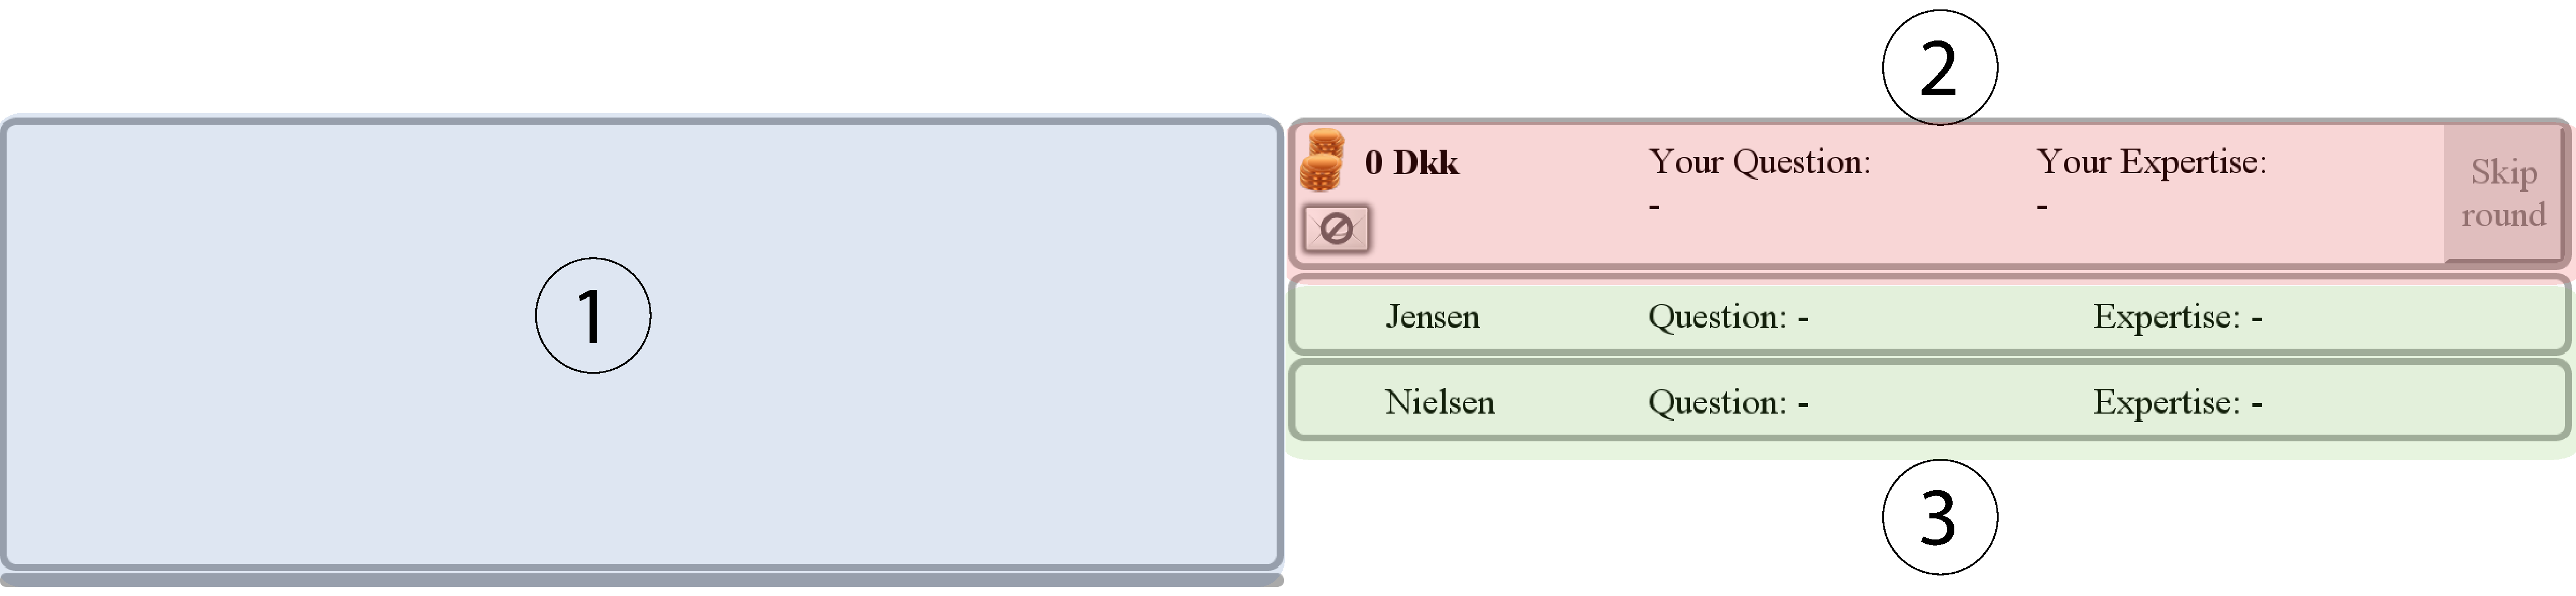
\includegraphics[width=\textwidth]{overview.pdf}\\
You are able to see:
 \begin{enumerate}
 \item \textcolor{blue}{Chat window}:  This is where the communication between you and a selected contact will show up
 \item \textcolor{red}{Your window}: Will indicate your own expertise and the question you are looking for
 \item \textcolor{green}{Contact list}: List of all other players.
 \end{enumerate}
 
 \subsection{New game}
 A new game will start automatically after you logged in.\\
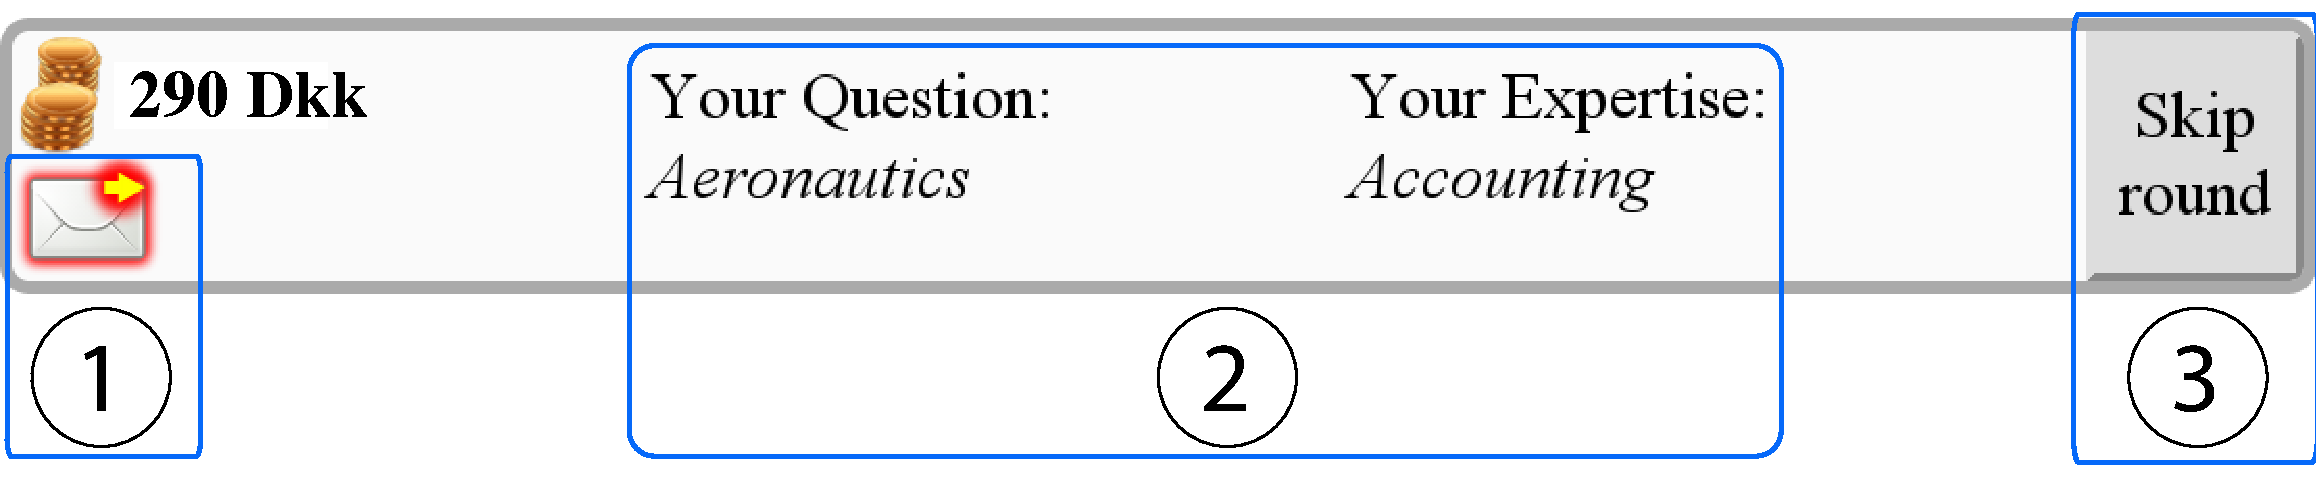
\includegraphics[width=\textwidth]{newGameUserWindow.pdf}\\

 You will notice some changes in \textcolor{red}{your window} once the game has started: 
  \begin{enumerate}
  \item Message indicator turns red, indicating that you are now able to send one message.
  \item In your window you are now able to see the expertise and question you were assigned for this game. 
   \item  If you don't want to send a message, in this round, click the skip button.
  \end{enumerate}
 \subsection{Sending an inquiry}
 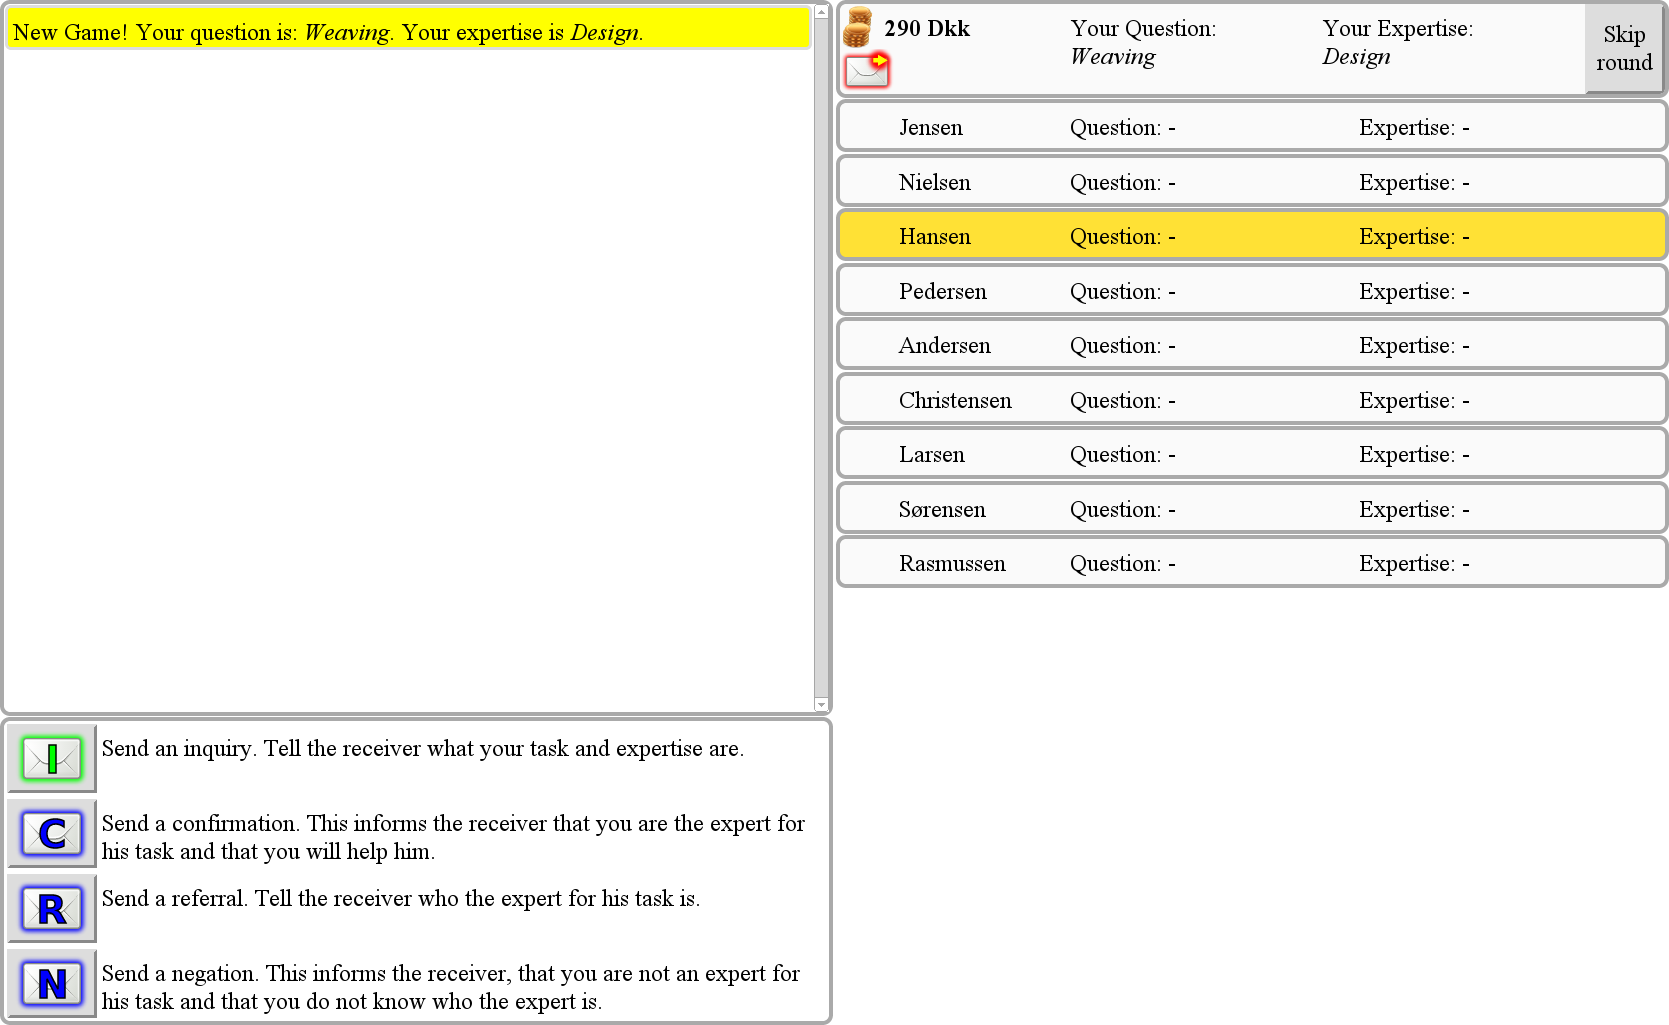
\includegraphics[width=\textwidth]{chatWindow.png}\\
Clicking on one of the names in the \textcolor{green}{Contact list} shows the communication between you and the contact that you clicked, in the \textcolor{blue}{Chat window}.
The selected contact is highlighted in Yellow. \\ 
At the bottom of the \textcolor{blue}{Chat window} you see buttons for the types of messages you can send to the selected contact.\\       
Clicking on the icon notice two things: \\
1) The inquiry you send is now displayed in the \textcolor{blue}{Chat window}\\
2) The message indicator is now turned grey.\\
After sending a message you have to wait for the round to end.
 \subsection{Receiving messages}
  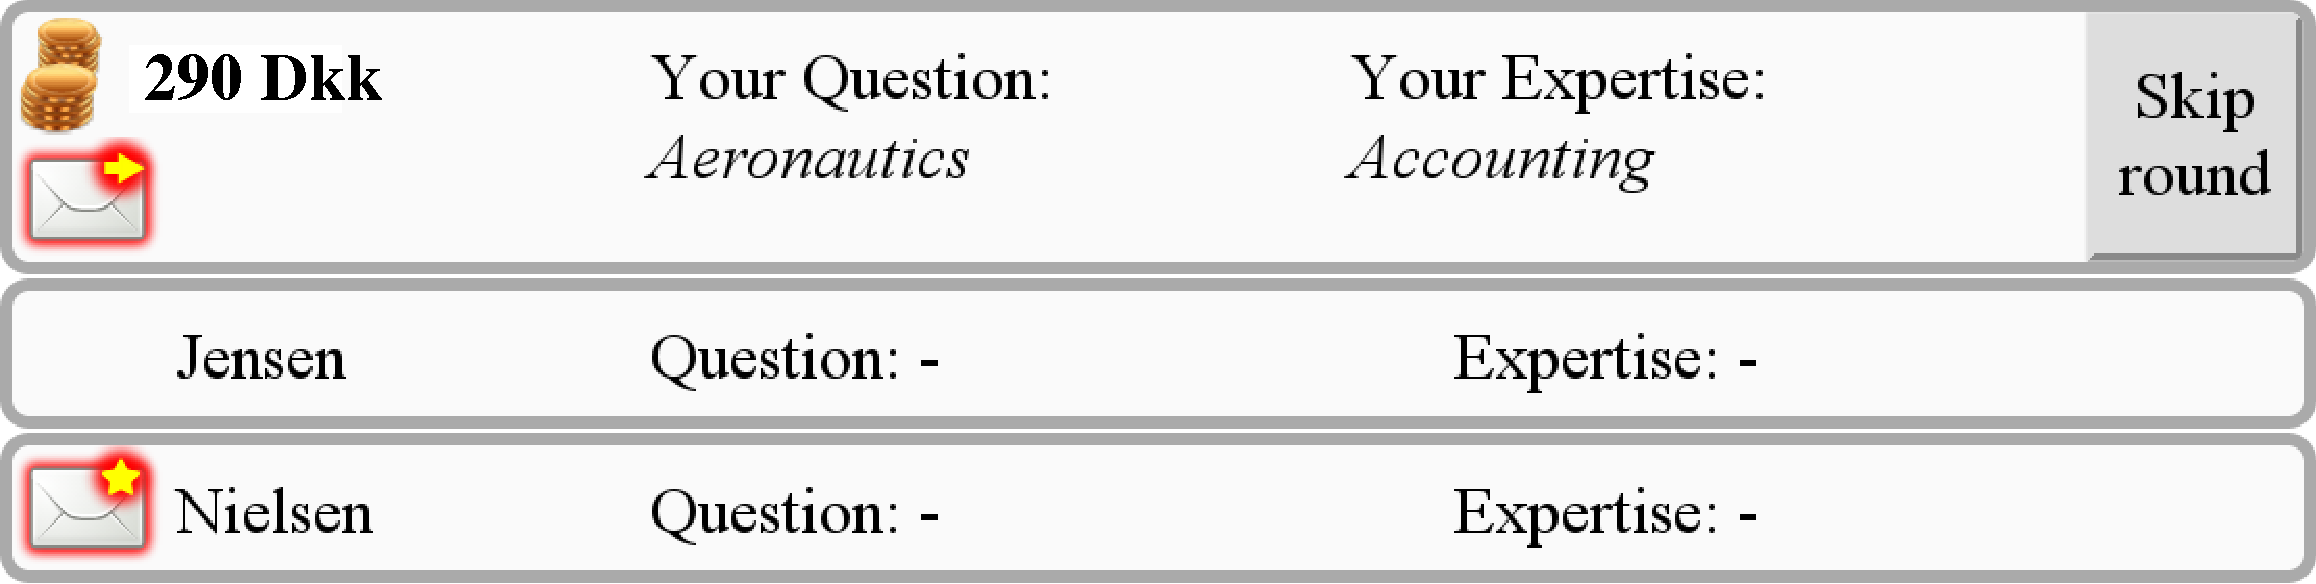
\includegraphics[width=\textwidth]{receiveMessageContactList.pdf}\\
At the beginning of a new round, the messages sent in the last round are delivered.\\ 
If you receive a message, "the new message" will show up as a new message icon 
\includegraphics[width=0.05\textwidth]{Unread.pdf} in the \textcolor{green}{Contact list}.\\
Clicking on the contact shows the contact's \textcolor{blue}{Chat window}, which contains the new message.\\
NOTICE, that the contacts question and expertise has now changed in the \textcolor{green}{Contact list}.  
 \subsection{Sending replies}
 If a contact, that has previously sent you a inquiry, is selected, you are able to reply by selecting the correct reply button in the \textcolor{blue}{Chat window}. \\
 Depending on your information, one of three different types of replies is possible:
   \begin{description}
  \item[\ActionC] 
\includegraphics[width=0.05\textwidth]{Confirm.pdf} A confirmation informs the receiving player, that you are his expert and that you will help him. The receiving player earns \Money{20 kr.}. You can only send a confirmation to another player if you know that you are his expert.
 \item[\ActionR] 
\includegraphics[width=0.05\textwidth]{Refer.pdf} A referral informs the receiving player who his expert is. You can only send a referral to another player if you know who his expert is, but it is not you.
 \item[\ActionN] 
\includegraphics[width=0.05\textwidth]{Negate.pdf} A negation informs the receiving player that you don't know who his expert is.
 \end{description}
 
 \subsection{Earning Money}
If you received a confirmation from your expert your money counter 
\includegraphics[width=0.05\textwidth]{Money.pdf} increases by \Money{20 kr}. Receiving multiple confirmations in the same game does NOT increase your earnings.    
   \section{Notes}
 You are given a form with the names of all players arranged in a circle and yourself in the middle. For every message you send to another player, please draw an arrow from ``You'' to the players name and indicate the type of message you sent with the letter specified in the top left corner of the form. For every message you receive from another player draw an arrow from the players name to ``You''. Use a new form for each game.
 
 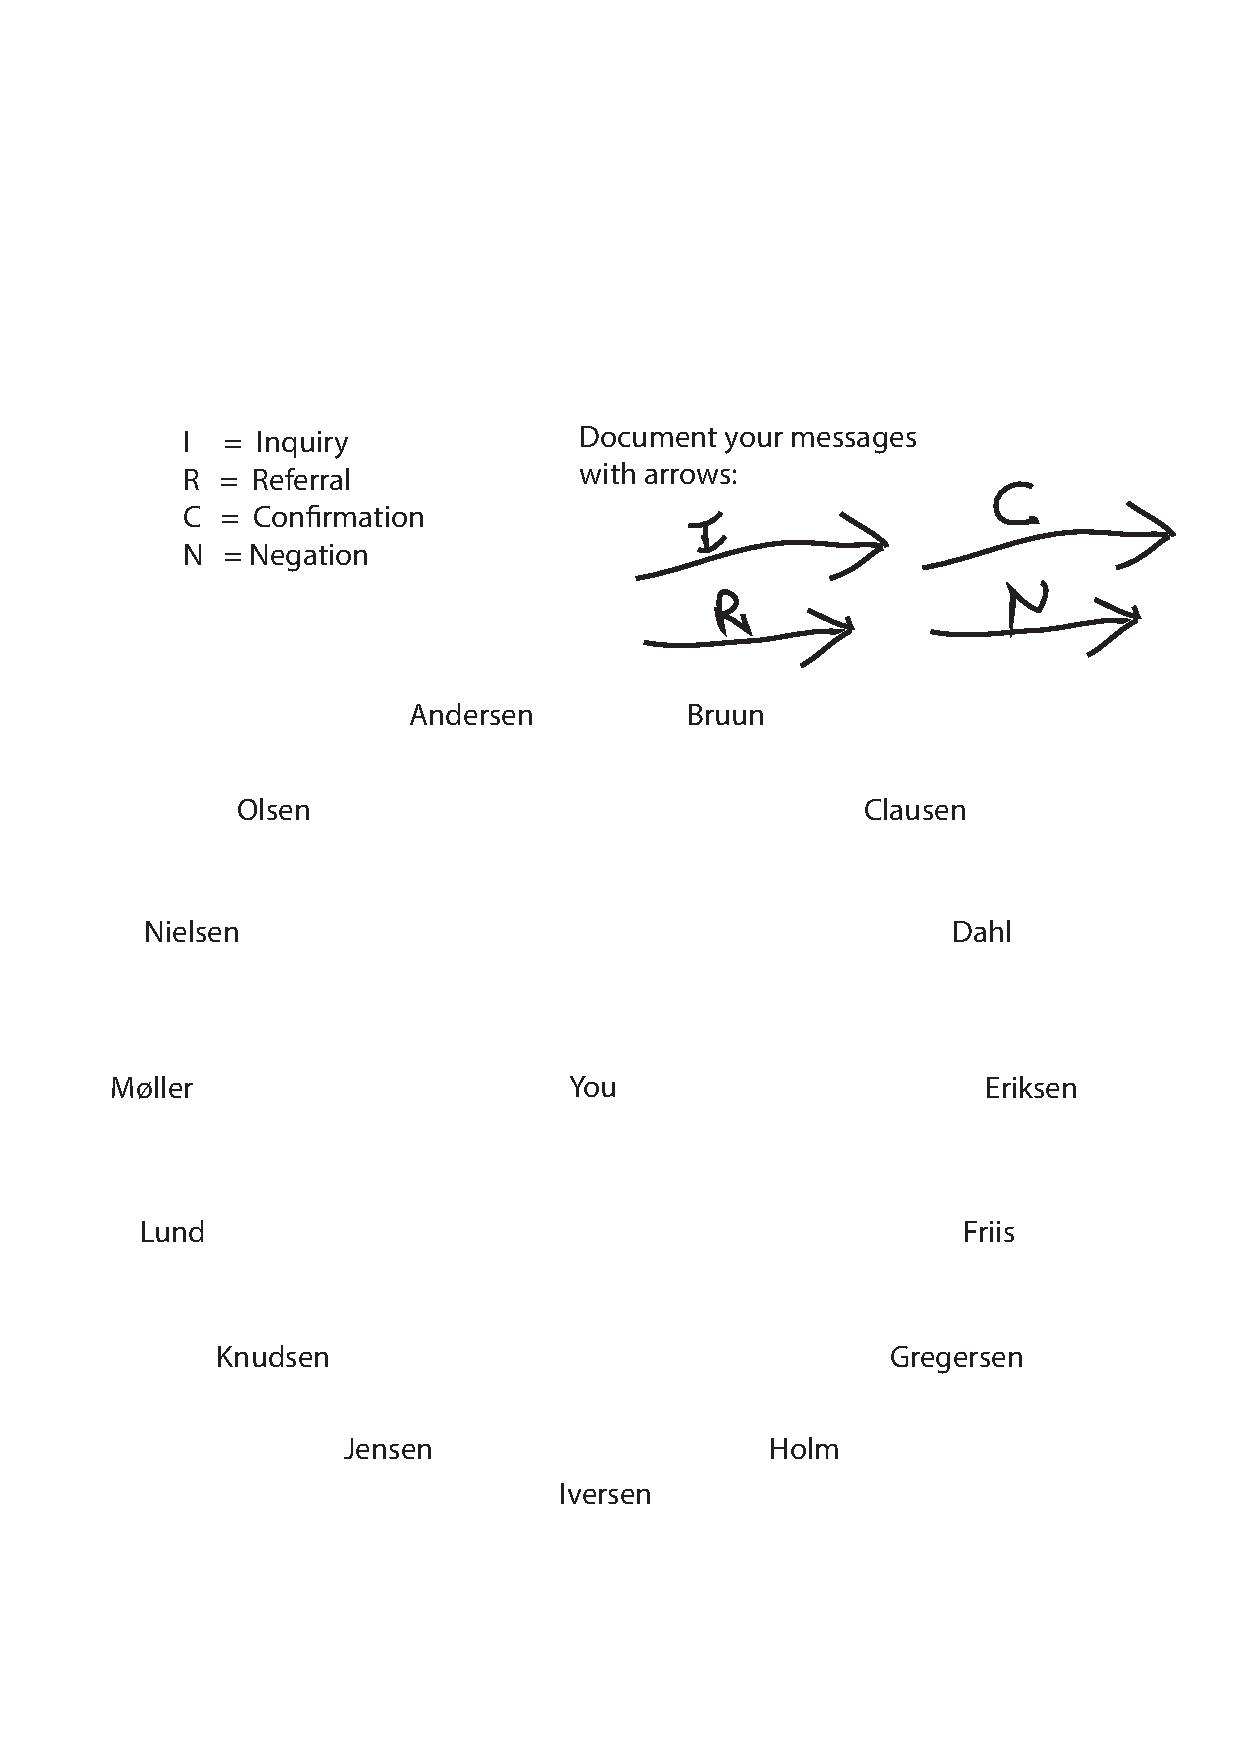
\includepdf{form.pdf}
  \end{document}
  
  
 
